\documentclass{article}

\usepackage{graphicx}
\usepackage{tikz}
\usepackage{tikzsymbols}
\usetikzlibrary{calc,patterns,shapes.geometric}
\pagestyle{empty}
\usepackage[margin=0pt]{geometry}
\geometry{papersize={14in,12in}}

\def\centerarc[#1](#2)(#3:#4:#5){\draw[#1] ($(#2)+({#5*cos(#3)},{#5*sin(#3)})$) arc (#3:#4:#5);}

\begin{document}
	\begin{figure}
		\centering
		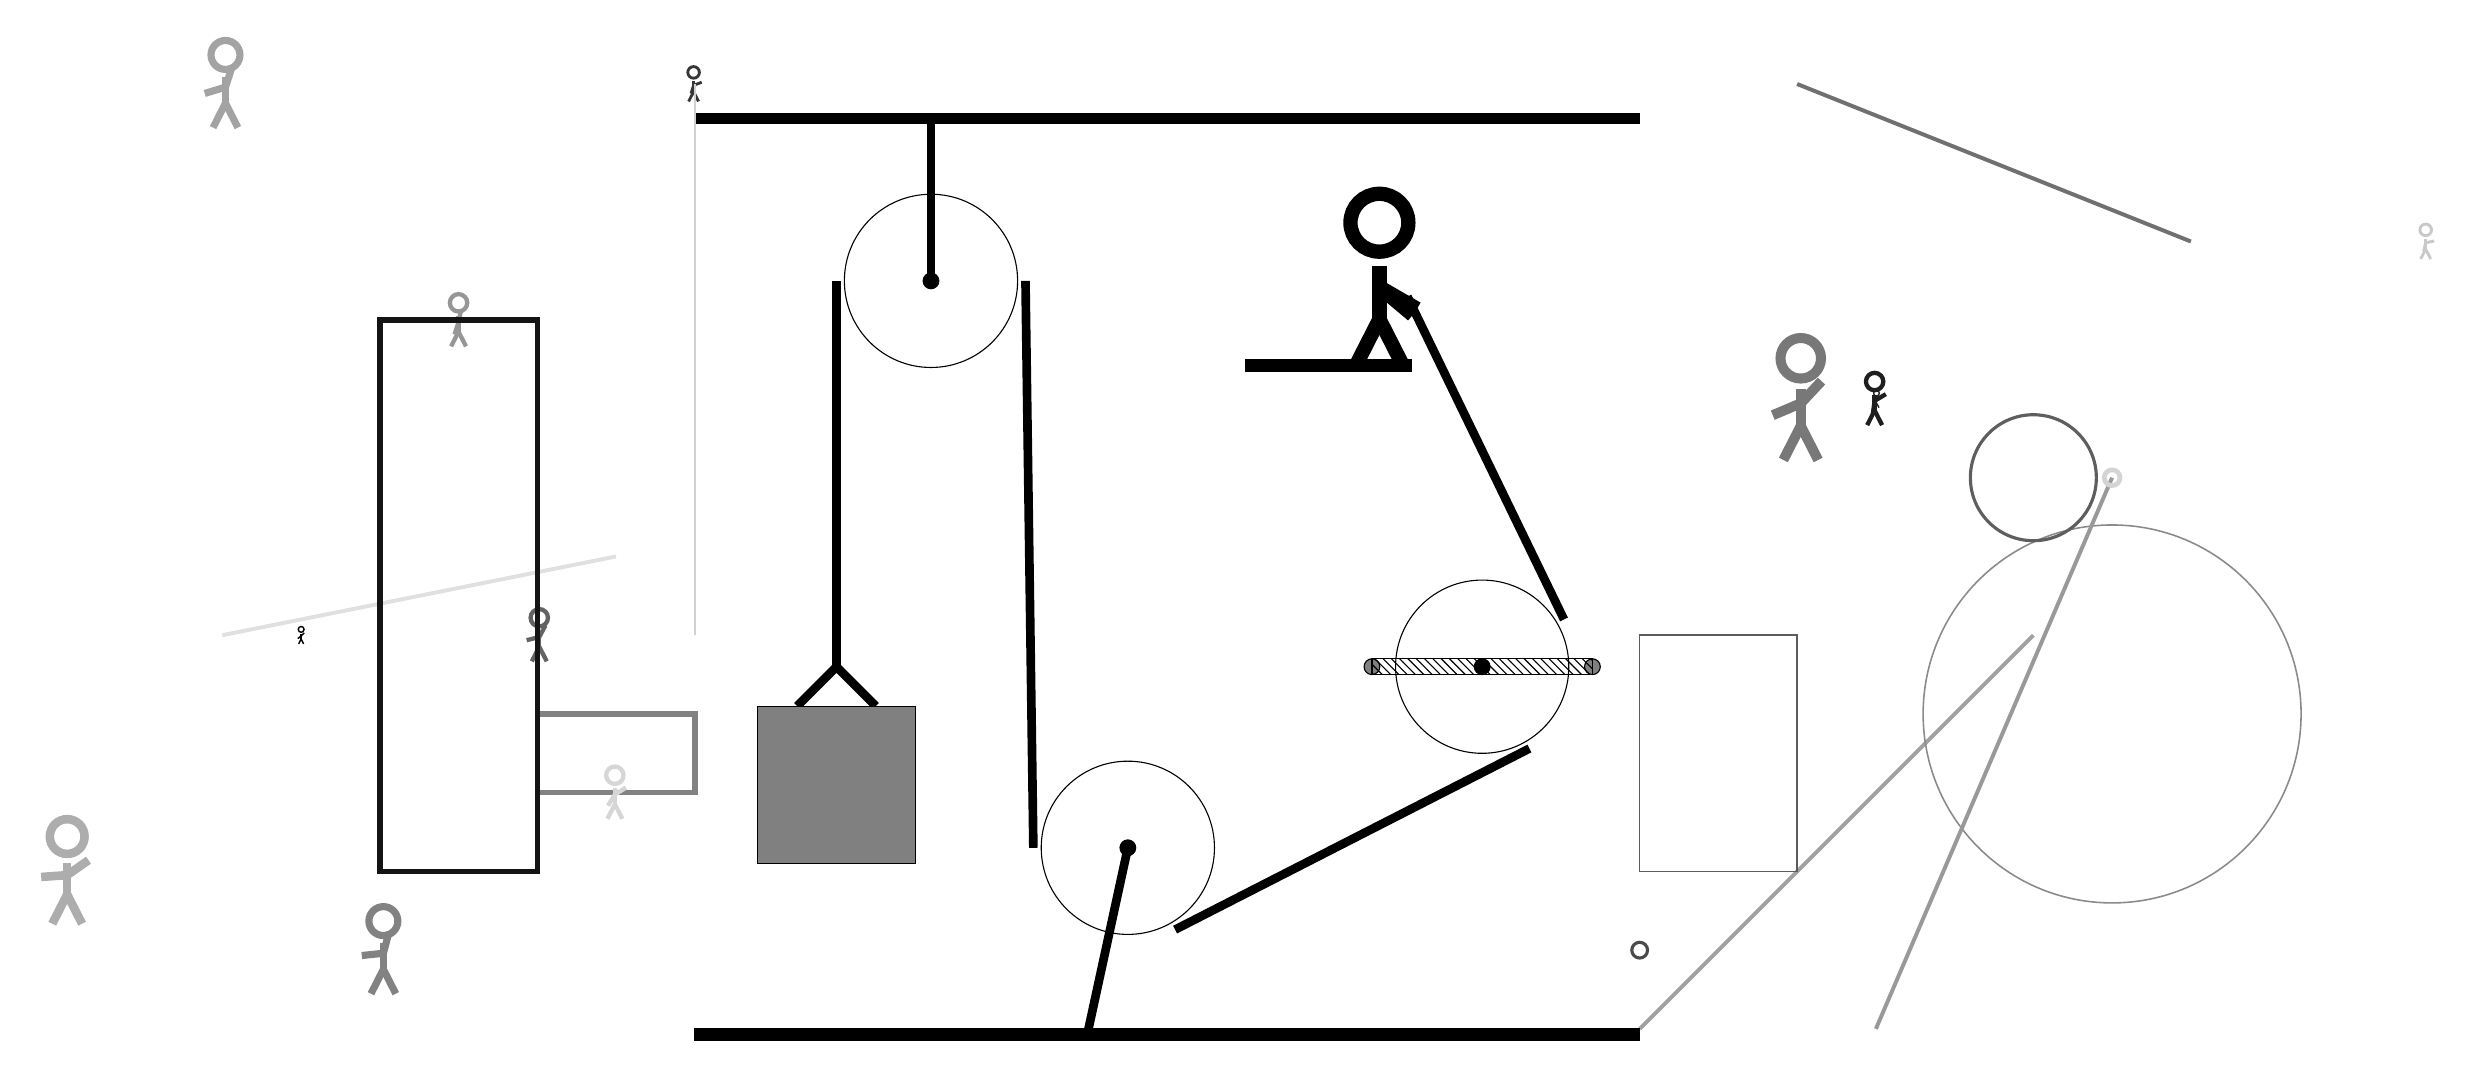
\begin{tikzpicture}
			%%%%% START %%%%%
			
			\draw[fill=black] (-2, 11.5) rectangle (10, 11.625);
			
			\draw (1, 9.5) circle (1.1);
			\draw[fill=black] (1, 9.5) circle (0.1);
			\draw[line width=1.1mm] (1, 11.5) -- (1, 9.5);
			
			\node[line width=0.2mm, color=black!61] at (-4, 5) {\Strichmaxerl[3][14][62]};
			
			\draw[line width=0.5mm, color=black!37](10, 0) -- (15, 5);
			\draw[line width=0.7mm, color=black!49] (-4, 4) rectangle (-2, 3);
			\node[line width=0.4mm, color=black!79] at (-2, 12) {\Strichmaxerl[2][73][20]};
			\draw [line width=0.4mm, color=black!71](10, 1) circle (0.1);
			\draw[line width=0.5mm, color=black!12](-3, 6) -- (-8, 5);
			\node[line width=0.2mm, color=black!98] at (-7, 5) {\Strichmaxerl[1][40][43]};
			\draw[line width=0.2mm, color=black!64] (12, 5) rectangle (10, 2);
			\draw [line width=0.2mm, color=black!46](16, 4) circle (2.4);
			
			\node[line width=0.7mm, color=black!36] at (-8, 12) {\Strichmaxerl[5][17][72]};
			\node[line width=0.7mm, color=black!85] at (13, 8) {\Strichmaxerl[1][21][62]};
			
			\node[line width=0.7mm, color=black!21] at (20, 10) {\Strichmaxerl[2][76][12]};
			\node[line width=0.2mm, color=black!41] at (-5, 9) {\Strichmaxerl[3][72][78]};
			
			\draw [line width=0.4mm, color=black!63](15, 7) circle (0.8);
			\node[line width=0.3mm, color=black!53] at (12, 8) {\Strichmaxerl[7][23][47]};
			\draw[line width=0.3mm, color=black!18] (-2, 12) rectangle (-2, 5);
			\node[line width=0.7mm, color=black!16] at (-3, 3) {\Strichmaxerl[3][58][32]};
			\draw[line width=0.5mm, color=black!40](13, 0) -- (16, 7);
			\node[line width=0.2mm, color=black!32] at (-10, 2) {\Strichmaxerl[6][4][35]};
			
			\node[line width=0.3mm, color=black!49] at (-6, 1) {\Strichmaxerl[5][6][75]};
			\draw[line width=0.7mm, color=black!92] (-4, 9) rectangle (-6, 2);
			
			\draw[line width=0.5mm, color=black!56](12, 12) -- (17, 10);
			\draw [line width=0.6mm, color=black!17](16, 7) circle (0.1);
			\draw [line width=0.2mm, color=black!31](-5, 1) circle (0.0);
			\node[line width=0.6mm, color=black!88] at (13, 8) {\Strichmaxerl[3][82][31]};
			
			\draw (3.5, 2.3) circle (1.1);
			\draw[fill=black] (3.5, 2.3) circle (0.1);
			\draw[line width=1.1mm] (3.5, 2.3) -- (3.0, 0);
			
			\draw[fill=white](8, 4.6) circle (1.1);
			\draw[fill=black] (8, 4.6) circle (0.1);
			\draw[fill=black!50] (9.4, 4.6) circle (0.1);
			\draw[fill=black!50] (6.6, 4.6) circle (0.1);
			\draw[pattern=north west lines, pattern color=black] (6.6, 4.7) rectangle (9.4, 4.5);
			
			\draw[line width=1.1mm](-0.7, 4.1) --  (-0.2, 4.6) -- (0.3, 4.1);
			\draw[fill=black!50] (-1.2, 4.1) rectangle (0.8, 2.1);
			
			\draw[line width=1.1mm](-0.2, 9.5) -- (-0.2, 4.6);
			\centerarc[line width=1.1mm](1, 9.5)(180:0:1.2000000000000002)
			\draw[line width=1.1mm](2.2, 9.5) -- (2.3, 2.3);
			\centerarc[line width=1.1mm](3.5, 2.3)(180:300:1.2000000000000002);
			\draw[line width=1.1mm](4.1, 1.2608) -- (8.6, 3.5608);
			\centerarc[line width=1.1mm](8, 4.6)(300:390:1.2000000000000002);
			\draw[line width=1.1mm](9.0392, 5.2) -- (7.05, 9.3);
			
			\node at (6.75, 9.5) {\Strichmaxerl[10][-220][-30]};
			\draw[fill=black] (5, 8.5) rectangle (7.1, 8.35);
			
			\draw[fill=black] (-2, 0) rectangle (10, -0.15);
			
			%%%%% END %%%%%
		\end{tikzpicture}
	\end{figure}	
\end{document}